\subsection{Shielding multi-process applications}
\label{sec:sgx:shield:multiproc}

Many Linux applications use multi-process abstractions,
which are implemented using copy-on-write fork and in-kernel
IPC abstractions.
In SGX, the host OS is untrusted, and enclaves cannot share protected memory.
Fortunately, \graphene{} implements multi-process support
including \syscall{fork}, \syscall{execve}, signals, and a subset of IPC mechanisms,
using message passing instead of shared memory.
%The {\it zero-sharing} nature of \graphene{} makes it possible
Thus, \graphenesgx{} implements multi-process abstractions in enclaves
without major library OS changes.
This subsection explains how
%we will describe how \graphenesgx{} securely creates
\graphenesgx{} protects
multi-processing abstractions from an untrusted OS.


%% \fixme{need to polish this subsection}

%% Upon existing platforms using \sgx{}, there is no
%% multi-process abstractions of any kinds that has been supported so far,
%% either in \haven{} or other systems.
%% The main challenge against
%% implementing multi-process abstractions in enclaves
%% is to share enclave pages,
%% for either Linux-style copy-on-write {\tt fork}'ing or
%% sharing abstraction states.
%% Fortunately,


%processes in new enclaves,
%%for supporting
%        {\tt fork}, {\tt execve},
%and inter-process communication
%(namespace coordination, signals, System V IPC, etc)
%with process isolation.

%\subsubsection{Forking into new enclaves}
%\label{sec:multiproc:fork}

\begin{figure}[t!]
\centering
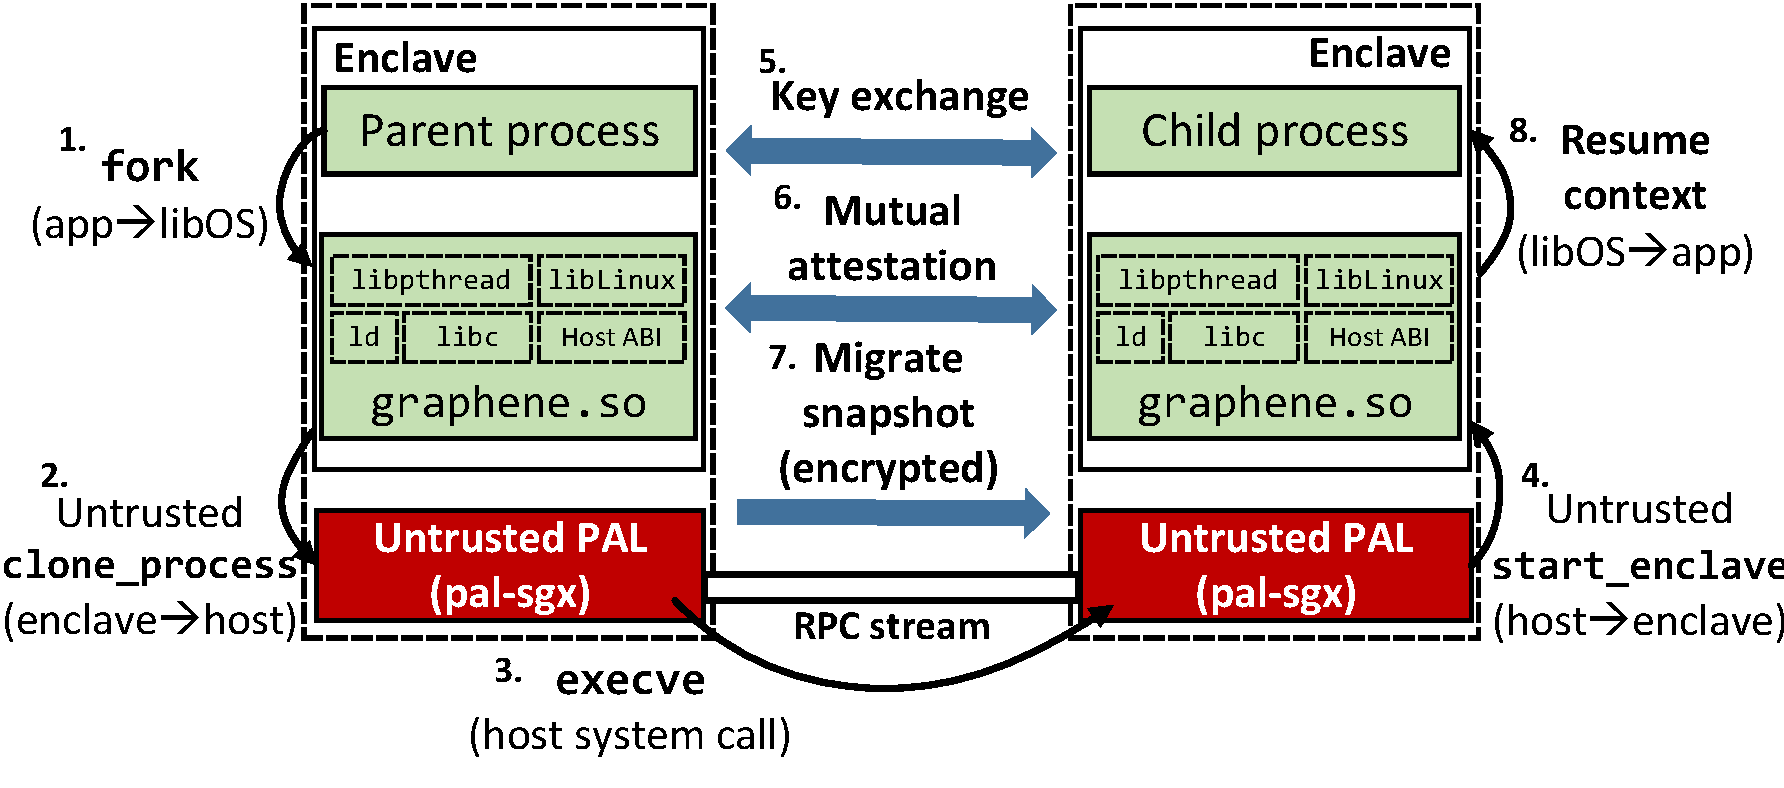
\includegraphics[width=34em]{fork.pdf}
\caption{Process creation in \graphenesgx{}.
Numbers show the order of operations.
When a process forks, \graphenesgx{} creates a new, clean enclave
%calls {\tt execve} system call
on the untrusted host.
%to create a clean enclave with the same \libos{} image.
Then the two enclaves %build up the mutual trust by
exchange an encryption key, validates the CPU-generated attestation of each other,
and migrates the parent process snapshot.}
\label{fig:sgx:fork}
\end{figure}

\begin{comment}
To secure process creation across enclaves,
\graphenesgx{} is capable of building up the trust to newly launched enclaves,
through cooperation with an untrusted host.
Once a clean and trusted new enclave is launched,
The parent process will send a snapshot to the new one,
to create a clone of itself.
Snapshotting and migrating process states
is a feature robustly implemented and heavily used in \graphene{} \libos{},
of which we simply inherit the design.
\end{comment}

Process creation in \graphenesgx{} is illustrated in Figure~\ref{fig:sgx:fork}.
When a process in \graphenesgx{} forks into a new enclave,
the parent and child will be running the same manifest and binaries,
and will have the same measurements.
%\fixme{rewrite this part. check this. dp: check my rewrite}
Similar to the process creation in Graphene, the parent and child enclaves are connected with a pipe-like RPC stream, through the untrusted PAL.
As part of initialization, the parent and child will exchange a session key over the unsecured RPC stream, using Diffie-Hellman.
The parent and child use the CPU to generate attestation reports, 
which include a 
512-bit field in the report to store 
a hash of the session key
and a unique enclave ID.
The parent and child exchange these reports to authenticate each other.
Unlike remote attestation, local attestation does not require 
use of Intel's authentication service (IAS).
% then exchange attestation reports \fixmedp{right?} generated by the CPU (unlike remote attestation, local attestation does not require Intel-owned services to verify the CPU).
% which will prove that the attested enclave is the one and only one that agrees on the key.
% sensitive data from being divulged to an attacker during \syscall{fork}.
%For example, to prevent a man-in-the-middle attack, between the parent and child,
%we use
%a 512-bit field
%in the CPU-signed attestation to store a hash of the session key
%and a unique enclave ID, which will prove that the attested enclave is the one and only one that agrees on the key.
%generated and signed by \sgx{}.
%Once the child enclave is launched, as part of initialization,
%the parent and child will exchange attestation generated by the CPU,
%exchange a signed session key using Diffie-Hellman, and then 
%establish a TLS connection over an inter-enclave RPC stream.
% after creating a signed session key using a key exchange algorithm like Diffie-Hellman.
%then use a session key to generate an encrypted connection.
%\fixmedp{I still don't understand the following text; let's discuss}
%What the Intel CPU provides here is the confidential CPU secret that the inter-enclave attestation is based on. The attestation establishes a trusted path within enclave groups to exchange library OS state.
%\fixmedp{IF time, clarify what HW provides here or how it works}
Once the parent and child have authenticated each other, the parent establishes a TLS connection over the RPC stream using the session key.
The parent can then send a snapshot of itself over
the TLS-secured RPC stream, and the snapshot is resumed in the child process, making it a clone of its parent.
This strategy
% between the parent and child
prevents a man-in-the-middle attack between the parent and child.
%To build up the trust, the two processes will open an encrypted channel
%using a session key,
%and exchange attestation generated by the processor.
%Once both sides have confirmed the integrity of the other,
%the parent process is safe to send its snapshot, encrypted, to the child
%through the said channel.
%The child process will resume the snapshot in its own enclave,
%making it a clone of its parent.


%The fork design in \graphenesgx{} provides several security measures.
%First, mutual attestation and encryption between the parent and child
%prevent sensitive data from being divulged to an attacker during {\tt fork()}.
%To prevent a man-in-the-middle attack, between parent and child,
%we use
%a 512-bit field
%in the attestation structure generated and signed by \sgx{}.
%We use this field to store a SHA-256 hash of the session key,
%and a unique enclave ID,
%\fixmedp{also a piece of intuition missing here; let's discuss}
%to prove that the attested enclave is the one and only one that agrees on the key.

%% Forking in \graphenesgx{} mainly defends against 3 types of attacks
%% from the untrusted host:

%% \begin{compactenum}

%% \item The host pretends to be the child enclave, to expose the process snapshot
%% sent from the parent.

%% \item The host pretends to be the parent enclave, to compromise the
%% child process using a malicious process snapshot.

%% \item The untrusted host becomes a man-in-the-middle, which bounces
%% encrypted messages between the child and parent enclaves, with session keys
%% negotiated with both sides.

%% \end{compactenum}

%% As described earlier, attacks 1 and 2 are prevented by mutual attestation
%% between the parent and the child,
%% and encrypting the channel for sending the snapshot.
%% The attestation signed by the processor proves that both entities communicating
%% are valid \graphenesgx{} enclaves,
%% and encrypting the channel prevents the snapshot being eavesdropped or
%% counterfeited by the host.

%% To defend against attack 3 (the man-in-the-middle attack), we take advantage of
%% a user-customized 512-bit field
%% in the attestation structure generated and signed by \sgx{}.
%% This field is filled with a SHA-256 hash value of the agreed session key,
%% and the current enclave ID,
%% to prove that the attested enclave is the one who agrees on the key.

Once a parent enclave forks a child, by default, the child is fully trusted.
To create a less trusted child, the parent would need to sanitize its snapshot,
similar in spirit to the close-on-exec flag for file handles.
%to maintain its own security,
%because the migrated snapshot discloses all information in the parent.
%Unless the binary run in the parent enclave ensures
%that no secrets is stored in the enclave memory at the time of snapshotting,
%the parent enclave cannot simply drop the trust against the child.
For example, a pre-forked Apache server may keep worker
processes isolated from the master %\fixmedp{Right nomenclature}, %that responds to HTTP requests isolated,
to limit a potential compromise of a worker process. %avoid being compromised by one attacked worker.
\graphenesgx{} inherits a limited API from \graphene{}, 
for applications to 
isolate themselves from untrusted child processes,
%\graphenesgx{} inherits this dynamic process isolation feature.
but applications are responsible for purging confidential information
before isolation.

\paragraph{Supporting \syscall{execve}.}

Unlike \syscall{fork}, \syscall{execve} 
starts a process with a specific executable, often different from the caller.
When a thread calls \syscall{execve} in \graphenesgx{},
the \libos{} migrates the thread to a new process,
with file handles being inherited.
%with clean process states except opened files cloned from the parent.
Although the child does not inherit a snapshot from its parent,
it can still compromise the parent 
by exploiting potential vulnerabilities in handling RPC, 
which are not internally shielded.
In other words, \graphenesgx{} is not designed to share library OS-internal
with untrusted children.
Thus, \graphenesgx{} restricts \syscall{execve} to only launch trusted executables, which are
specified in the manifest.


%  main challenge to supporting \exec{} is to
%ensure only trusted binaries can be created as child processes.
%loaded into new enclaves as child processes.
%The trust between parent and child must be mutual,
%or applications won't be secure.
%unless the two enclaves are strictly isolated.
%To secure \exec{},
%\graphenesgx{} stores the enclave measurements of executable binaries that can be trusted as children processes
%inside the manifest file.
%To identify binaries that can be trusted (either as parents or children)
%during process creation,
%\graphenesgx{} requires each binary ported for an application,
%to be shipped with a list of binaries that can be \exec{}'d,
%and those that can be callers of \exec{} to the said binary.
%Each binary in the list is identified by its measurement, which is mutually attested
%between the parent and the child during process creation.
%This list must be signed by a private key provided by the client,
%while the public key must be included in the enclave measurement of the binary.


\paragraph{Inter-process communication.}
\label{sec:multiproc:ipc}

After process creation, parent and child processes will cooperate
through shared abstractions,
such as signals or System V message queues, via RPC messages.
While messages are being exchanged between enclaves,
they are encrypted, ensuring that these abstraction are protected
from the OS.

%For \libos{}, OS states for these shared abstractions must be shared
%though inter-process coordination, for mainly two purposes.
%First, for each abstraction, \libos{} needs to maintain the state
%in one of its instances.
%Second, \libos{} must maintain the namespace states to identify and locate the
%abstraction states.
%\graphene{} implements a wide range of multi-process abstractions and namespaces,
%by coordinating OS state over RPC streams, rather than using shared memory. 

%% dp: this point already made above
%Because SGX does not allow enclaves to share trusted memory,
%the fact that the original Graphene design did not require shared memory
%made porting to SGX considerably easier.

% (pipes).
%Such a design is perfect for porting multi-process applications to enclaves.

%Thus, by coordinating OS state via 
%Thus, the benefit of coordinating OS state via message passing 
%is that 
%the enclaves need no will not share any memory to
%coordinate abstraction states,
%simplifying the support and security of library OS.
%and the RPC streams can be secured by the enclaves instead of the host.
%By encrypting the RPC streams among related processes,
%inter-process communication is easily protected from the untrusted OSes.
%In \graphene{}, security isolation among multi-process abstractions,
%regardless of their semantics,
%are enforced by isolating the RPC streams used for coordination.
%Unfortunately, \graphenesgx{} cannot trust the host to faithfully isolate
%the RPC streams.
%Each enclave launched for an application must secure inter-process coordination
%spontaneously, by only communicating to enclaves that it has attested
%and exchanged secret keys with.
%Because inter-process coordination is completely transparent
%to the applications,
%all information sent over RPC streams must be encrypted,
%because \libos{} cannot determine whether the information may contain any secret.





